%%%%%%%%%%%%%%%%%%%%%%%%%%%%%%%%%%%%%%%%%
% Short Sectioned Assignment LaTeX Template Version 1.0 (5/5/12)
% This template has been downloaded from: http://www.LaTeXTemplates.com
% Original author:  Frits Wenneker (http://www.howtotex.com)
% License: CC BY-NC-SA 3.0 (http://creativecommons.org/licenses/by-nc-sa/3.0/)
%%%%%%%%%%%%%%%%%%%%%%%%%%%%%%%%%%%%%%%%%

%----------------------------------------------------------------------------------------
%	PACKAGES AND OTHER DOCUMENT CONFIGURATIONS
%----------------------------------------------------------------------------------------

\documentclass[paper=a4, fontsize=11pt]{scrartcl} % A4 paper and 11pt font size

% ---- Entrada y salida de texto -----

\usepackage[T1]{fontenc} % Use 8-bit encoding that has 256 glyphs
\usepackage[utf8]{inputenc}

% ---- Idioma --------

\usepackage[spanish, es-tabla]{babel} % Selecciona el español para palabras introducidas automáticamente, p.ej. "septiembre" en la fecha y especifica que se use la palabra Tabla en vez de Cuadro

% ---- Otros paquetes ----

\usepackage{amsmath,amsfonts,amsthm} % Math packages
\usepackage{graphics,graphicx, floatrow} %para incluir imágenes y notas en las imágenes
\usepackage{graphics,graphicx, float} %para incluir imágenes y colocarlas
\usepackage{hyperref} % url in references

% Para hacer tablas comlejas
\usepackage{multirow}
\usepackage{threeparttable}

\usepackage{fancyhdr} % Custom headers and footers
\pagestyle{fancyplain} % Makes all pages in the document conform to the custom headers and footers
\fancyhead{} % No page header - if you want one, create it in the same way as the footers below
\fancyfoot[L]{} % Empty left footer
\fancyfoot[C]{} % Empty center footer
\fancyfoot[R]{\thepage} % Page numbering for right footer
\renewcommand{\headrulewidth}{0pt} % Remove header underlines
\renewcommand{\footrulewidth}{0pt} % Remove footer underlines
\setlength{\headheight}{13.6pt} % Customize the height of the header

\numberwithin{equation}{section} % Number equations within sections (i.e. 1.1, 1.2, 2.1, 2.2 instead of 1, 2, 3, 4)
\numberwithin{figure}{section} % Number figures within sections (i.e. 1.1, 1.2, 2.1, 2.2 instead of 1, 2, 3, 4)
\numberwithin{table}{section} % Number tables within sections (i.e. 1.1, 1.2, 2.1, 2.2 instead of 1, 2, 3, 4)

\setlength\parindent{0pt} % Removes all indentation from paragraphs - comment this line for an assignment with lots of text

\newcommand{\horrule}[1]{\rule{\linewidth}{#1}} % Create horizontal rule command with 1 argument of height

\usepackage{textcomp}
\usepackage{hyperref}

%----------------------------------------------------------------------------------------
%	DATOS
%----------------------------------------------------------------------------------------

\newcommand{\myName}{Francisco Javier Bolívar Lupiáñez}
\newcommand{\myDegree}{Máster en Ingeniería Informática}
\newcommand{\myFaculty}{E. T. S. de Ingenierías Informática y de Telecomunicación}
\newcommand{\myDepartment}{Ciencias de la Computación e Inteligencia Artificial}
\newcommand{\myUniversity}{\protect{Universidad de Granada}}
\newcommand{\myLocation}{Granada}
\newcommand{\myTime}{\today}
\newcommand{\myTitle}{Práctica 1}
\newcommand{\mySubtitle}{Despliegue de MVs y Aplicaciones Web}
\newcommand{\mySubject}{Cloud Computing: Servicios y Aplicaciones}
\newcommand{\myYear}{2016-2017}

%----------------------------------------------------------------------------------------
%	PORTADA
%----------------------------------------------------------------------------------------


\title{	
	\normalfont \normalsize 
	\textsc{\textbf{\mySubject \space (\myYear)} \\ \myDepartment} \\[20pt] % Your university, school and/or department name(s)
	\textsc{\myDegree \\[10pt] \myFaculty \\ \myUniversity} \\[25pt]
	\horrule{0.5pt} \\[0.4cm] % Thin top horizontal rule
	\huge \myTitle: \mySubtitle \\ % The assignment title
	\horrule{2pt} \\[0.5cm] % Thick bottom horizontal rule
	\normalfont \normalsize
}

\author{\myName} % Nombre y apellidos

\date{\myTime} % Incluye la fecha actual
%----------------------------------------------------------------------------------------
%	INDICE
%----------------------------------------------------------------------------------------

\begin{document}
	
\definecolor{light-gray}{gray}{0.95}
	
\lstset {
	basicstyle=\scriptsize,
	frame=single,
	backgroundcolor=\color{grey}
}
	
\setcounter{page}{0}

\maketitle % Muestra el Título
\thispagestyle{empty}

\newpage %inserta un salto de página

\tableofcontents % para generar el índice de contenidos

%\listoffigures

\newpage

%----------------------------------------------------------------------------------------
%	DOCUMENTO
%----------------------------------------------------------------------------------------

\section{Introducción}

El objetivo de esta práctica es familiarizarse con el uso de una plataforma IaaS y desarrollar habilidades de despliegue de máquinas virtuales y aplicaciones web sencillas.
\\ \\
Para ello el alumno deberá realizar las tareas que se describen a continuación usando la plataforma OpenNebula:

\begin{itemize}
	\item Crear dos MVs, cada una con una distribución de Linux:
	\begin{itemize}
		\item En la primera MV instalar y configurar un servidor web.
		\item En la segunda MV instalar y configurar un sistema gestor de bases de datos (SGBD).
	\end{itemize}
	\item Desarrollar una aplicación web sencilla alojada en la MV1, que use una base de datos manejada por el SGBD instalado en al MV2. La aplicación web debe incluir el uso de formularios y la consulta y modificación de datos almacenados en la BD.
	\item Realizar el despliegue de ambas MVs, para evaluar el funcionamiento de la aplicación.
\end{itemize}

\label{sec:conexion}
\subsection{Conexión con OpenNebula}

Para conectarse con OpenNebula hay que hacerlo mediante ssh conectándose a la dirección \texttt{docker.ugr.es} con el usuario \texttt{mccDNI-SIN-LETRA}. Por ejemplo:

\begin{lstlisting}
ssh mcc12345678@docker.ugr.es
\end{lstlisting}

Una vez conectado escribir la siguiente orden: 

\begin{lstlisting}
oneuser login mccDNI-sin-LETRA --ssh --force
\end{lstlisting}

Y con: 

\begin{lstlisting}
more .one/one_auth
\end{lstlisting}

podemos obtener las credenciales para acceder a la plataforma desde la web \url{http://docker.ugr.es:9869}.

\section{Despliegue de máquinas virtuales}

El despliegue de máquinas virtuales se ha realizado mediante la interfaz de línea de órdenes de OpenNebula. Para ello hay que conectarse como se especificó en la sección \ref{sec:conexion}.

\label{sec:crear-plantilla}
\subsection{Crear plantilla}

Para crear una plantilla necesitamos información como el identificador de la imagen como la red propia del usuario.
\\ \\
Para encontrar el id de la imagen que se utilizará en la plantilla, listamos las imágenes disponibles con:

\begin{lstlisting}
oneimage list
\end{lstlisting}

\begin{figure}[H]
	\centering
	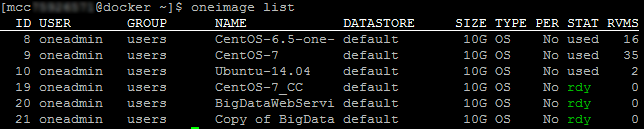
\includegraphics[width=14cm]{img/oneimage-list}
	\caption{Lista de imágenes disponibles}
	\label{fig:one-image-list}
\end{figure}

Y para dar con la red:

\begin{lstlisting}
onevnet list | grep mccDNI-SIN-LETRA
\end{lstlisting}

\begin{figure}[H]
	\centering
	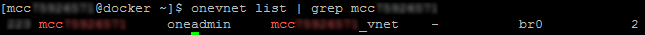
\includegraphics[width=14cm]{img/onevnet-list}
	\caption{Datos de red de un usuario específico}
	\label{fig:onevnet-list}
\end{figure}

Con estos datos ya podemos crear un template, por ejemplo:

\begin{lstlisting}
onetemplate create --name "Template_CentOS-7" --cpu 1 
--vcpu 1 --memory 1024 --arch x86_64 --disk 9 
--nic "MI-ID-RED" --vnc --ssh --net_context
\end{lstlisting}

Esto creará un template y le asignará un identificador único. Para consultarlo podemos listar nuestros templates con:

\begin{lstlisting}
onetemplate list
\end{lstlisting}

\begin{figure}[H]
	\centering
	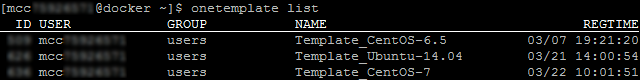
\includegraphics[width=14cm]{img/onetemplate-list}
	\caption{Lista de templates}
	\label{fig:onetemplate-list}
\end{figure}

\subsection{Desplegar máquina virtual}

Para crear una máquina virtual necesitaremos un template, cuyo ID podemos obtener como se ha explicado en la Sección \ref{sec:crear-plantilla}.
\\ \\
Tan solo hay que usar la orden:

\begin{lstlisting}
onetemplate instantiate ID
\end{lstlisting}

Esto instanciará e iniciará la máquina virtual pasando por distintos estados (Figura \ref{fig:grafo-estados}).

\begin{figure}[H]
	\centering
	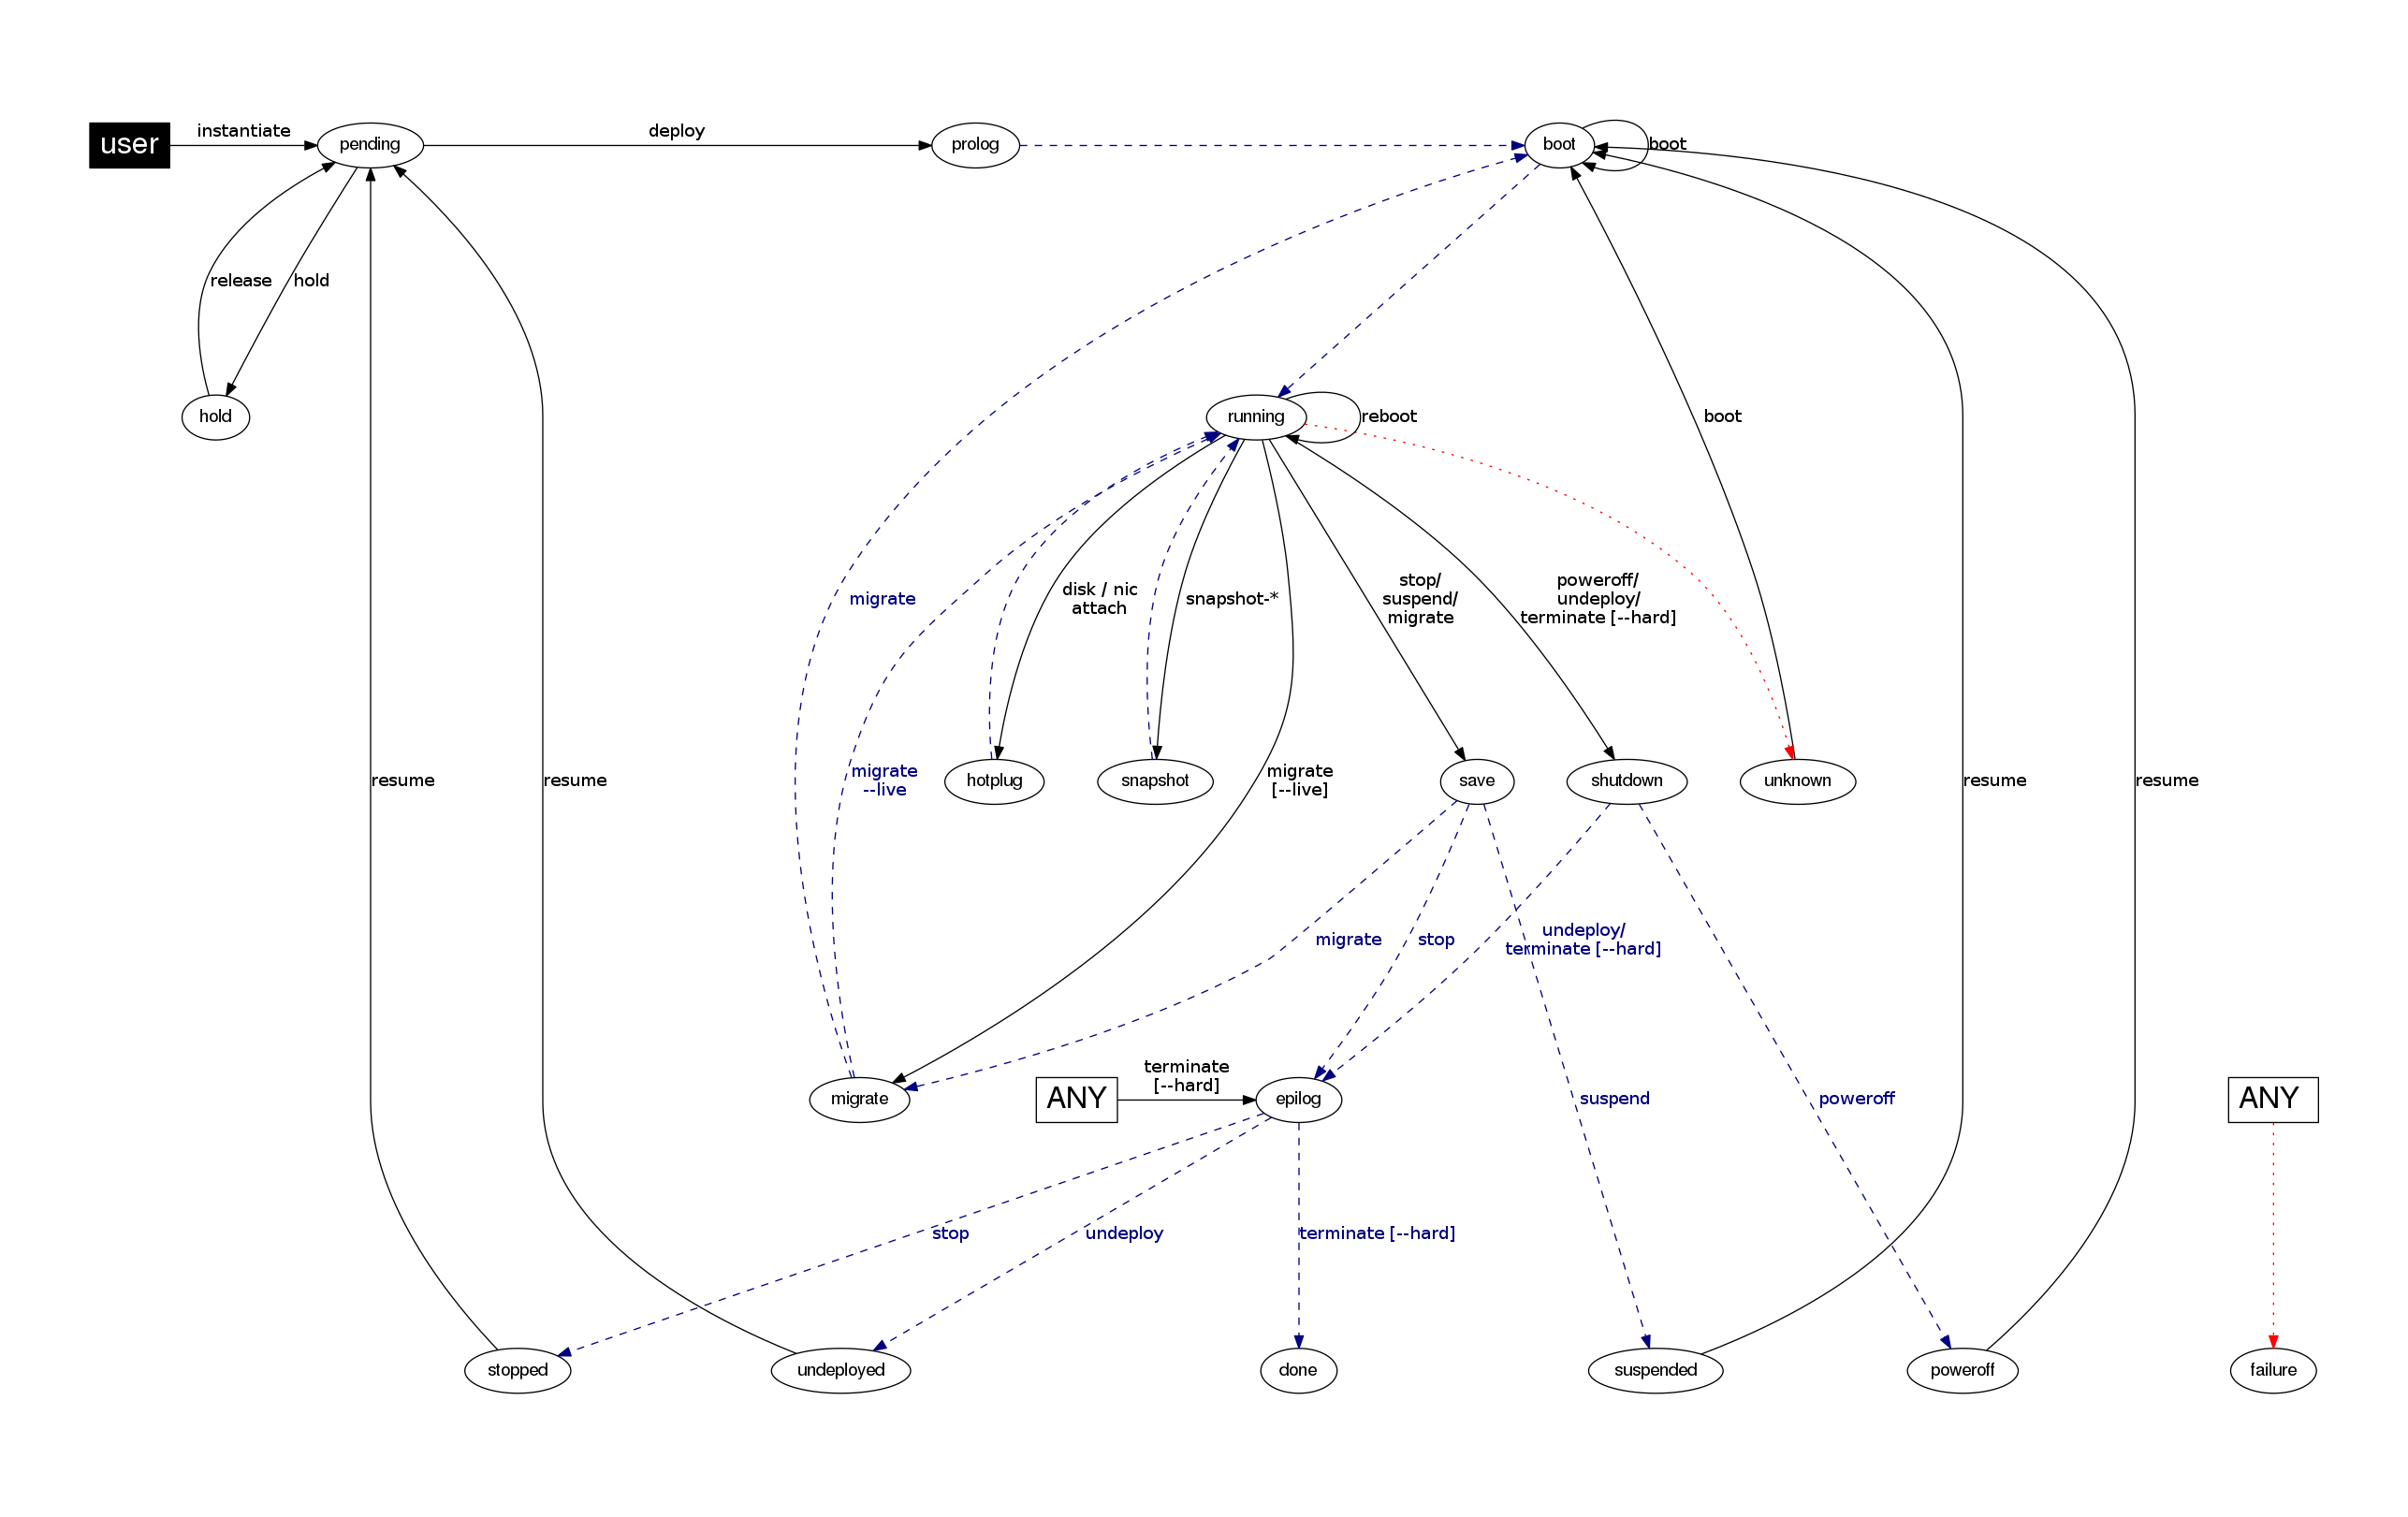
\includegraphics[width=14.5cm]{img/grafo-estados}
	\caption{Grafo de los estados por los que pasa una máquina virtual}
	\label{fig:grafo-estados}
\end{figure}

Para listar las máquinas virtuales usaremos:

\begin{lstlisting}
onevm list
\end{lstlisting}

\begin{figure}[H]
	\centering
	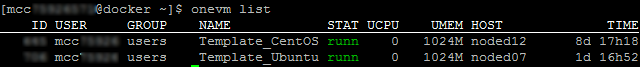
\includegraphics[width=14cm]{img/onevm-list}
	\caption{Lista de máquinas virtuales}
	\label{fig:onevm-list}
\end{figure}

La información de una máquina virtual específica la podemos consultar con:

\begin{lstlisting}
onevm show ID
\end{lstlisting}

De aquí podemos obtener la dirección IP (\texttt{ETH0\_IP}) para conectarse posteriormente a ella vía ssh:

\begin{figure}[H]
	\centering
	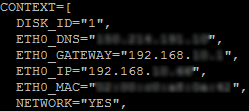
\includegraphics[width=5cm]{img/onevm-show-context}
	\caption{Direcciones de red de una máquina virtual}
	\label{fig:onevm-show-context}
\end{figure}

\section{SGBD}

\subsection{CentOS 7}

Usaremos una máquina virtual con CentOS 7 para alojar nuestro SGBD (MariaDB). Para ello seguiremos los pasos de un tutorial de DigitalOcean \cite{InstallMariaDBCentos7} con los que instalaremos MariaDB.
\\ \\
Para comenzar nos conectamos a la máquina virtual mediante ssh con \texttt{ssh root@ETH0\_IP} y lo primero que haremos será actualizar el sistema con:

\begin{lstlisting}
yum update
\end{lstlisting}

Ahora instalaremos Apache con:

\begin{lstlisting}
yum install mariadb-server
\end{lstlisting}

Una vez instalado se puede lanzar usando:

\begin{lstlisting}
systemctl start mariadb
\end{lstlisting}

Para que se inicie el servicio cada vez que se inicie el sistema:

\begin{lstlisting}
systemctl enable mariadb
\end{lstlisting}

Una vez instalado podemos cargar la base de datos cargando el script que se encuentra en \url{https://github.com/fblupi/starsator-db} con la siguiente orden:

\begin{lstlisting}
mysql < stars.sql
\end{lstlisting}

\section{Servidor web}

En esta sección se explicará como montar el servidor web tanto en CentOS 7 como en Ubuntu 14.04.

\subsection{CentOS 7}

Usaremos otra máquina virtual con CentOS 7 para alojar nuestro servidor web (Apache). Para ello seguiremos los pasos de un tutorial de DigitalOcean \cite{InstallLAMPCentos7} con los que instalaremos Apache y PHP e ignorando los pasos para instalar MariaDB pues, recordamos, esta máquina virtual solo contendrá el servidor web.
\\ \\
Para comenzar nos conectamos a la máquina virtual mediante ssh con \texttt{ssh root@ETH0\_IP} y lo primero que haremos será actualizar el sistema con:

\begin{lstlisting}
yum update
\end{lstlisting}

Ahora instalaremos Apache con:

\begin{lstlisting}
yum install httpd
\end{lstlisting}

Una vez instalado se puede lanzar usando:

\begin{lstlisting}
systemctl start httpd.service
\end{lstlisting}

Para que se inicie el servicio cada vez que se inicie el sistema:

\begin{lstlisting}
systemctl enable httpd.service
\end{lstlisting}

Ahora abrimos el puerto para permitir el tráfico por HTTP:

\begin{lstlisting}
firewall-cmd --permanent --zone=public --add-service=http
firewall-cmd --reload
\end{lstlisting}

Por último instalamos PHP pues la aplicación web está desarrollada con esta tecnología. Para ello ejecutamos:

\begin{lstlisting}
yum install php php-mysql
\end{lstlisting}

Una vez instalado podemos cargar los fuentes en el directorio \texttt{/var/www/html/}. Yo los he obtenido clonando mi repositorio de GitHub donde están alojados: \url{https://github.com/fblupi/starsator-web}.

\subsection{Ubuntu 14.04}

Alternativamente podemos usar una máquina virtual con Ubuntu 14.04 para alojar nuestro servidor web (Apache). Para ello seguiremos los pasos de un tutorial de DigitalOcean \cite{InstallLAMPUbuntu14.04} con los que instalaremos Apache y PHP e ignorando los pasos para instalar MySQL pues, recordamos, esta máquina virtual solo contendrá el servidor web.
\\ \\
Para comenzar nos conectamos a la máquina virtual mediante ssh con \texttt{ssh root@ETH0\_IP} y lo primero que haremos será actualizar el sistema con:

\begin{lstlisting}
apt-get update && apt-get upgrade
\end{lstlisting}

Ahora instalaremos Apache con:

\begin{lstlisting}
apt-get install apache2
\end{lstlisting}

Una vez instalado se puede lanzar usando:

\begin{lstlisting}
service apache2 start
\end{lstlisting}

A diferencia de CentOS, en Ubuntu ya tendremos por defecto abierto el puerto 80, por lo que no habrá que abrirlo manualmente.
\\ \\
Por último instalamos PHP pues la aplicación web está desarrollada con esta tecnología. Para ello ejecutamos:

\begin{lstlisting}
apt-get install php php-mysql
\end{lstlisting}

Para usar el \texttt{index.php} en lugar del \texttt{index.html} alojado en la raíz del servidor, hay que editar el fichero \texttt{/etc/apache2/mods-enabled/dir.conf} y dejarlo así:

\begin{lstlisting}
<IfModule mod_dir.c>
  DirectoryIndex index.php index.html index.cgi index.pl index.xhtml index.htm
</IfModule>
\end{lstlisting}

Una vez instalado podemos cargar los fuentes en el directorio \texttt{/var/www/html/}. Yo los he obtenido clonando mi repositorio de GitHub donde están alojados: \url{https://github.com/fblupi/starsator-web}.

\section{Conectar ambas máquinas virtuales}

Para acceder al puerto 80 de una de las máquinas virtuales dentro de \texttt{docker.ugr.es} tenemos que acceder por el puerto 150XX donde XX son los dos últimos dígitos de la dirección IP de la máquina virtual en la red privada.
\\ \\
Para acceder a la máquina virtual con el SGBD desde la del servidor web, al estar en la misma red privada, se podrá hacer directamente accediendo desde el puerto 3306.

\begin{figure}[H]
	\centering
	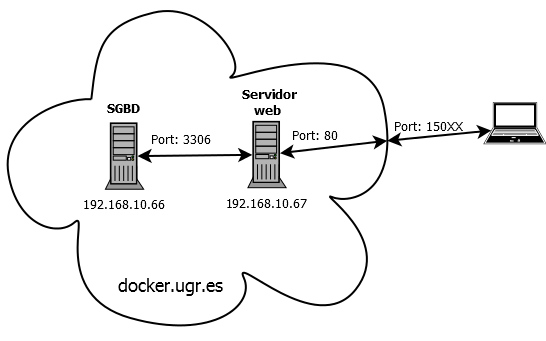
\includegraphics[width=11cm]{img/esquema-red}
	\caption{Esquema de conexiones de red}
	\label{fig:esquema-red}
\end{figure}

\subsection{SGBD}
\label{sec:conectar-mvs-sgbd}

Hay que realizar una serie de pasos para configurar el SGBD para que sea accesible desde una dirección IP remota \cite{EnableRemoteAccessToMariaDB}.
\\ \\
En primer lugar hay que dar acceso a la dirección IP remota:
\\ \\
\begin{lstlisting}
mysql
GRANT ALL PRIVILEGES ON starsator.* TO 'web'@'192.168.10.XX' 
  IDENTIFIED BY 'password' WITH GRANT OPTION;
exit;
\end{lstlisting}

Para ello hay que abrir el puerto usando la orden:

\begin{lstlisting}
firewall-cmd --add-port=3306/tcp 
firewall-cmd --permanent --add-port=3306/tcp
\end{lstlisting}

Y finalmente se reinicia el servicio: 

\begin{lstlisting}
systemctl restart mariadb
\end{lstlisting}

\subsection{Servidor web}

Para que nuestra aplicación web acceda a la base de datos del SGBD hay que editar el archivo \texttt{dbConnection.php} que se encuentra en \texttt{php/script} editando las siguientes variables \cite{PHPRemoteMySQLConnection}:

\begin{itemize}
	\item \texttt{servername}: Dirección IP en la red local de la máquina virtual donde se aloja el SGBD (192.168.10.XX).
	\item \texttt{username}: Nombre de usuario al que hemos dado privilegios en la Sección \ref{sec:conectar-mvs-sgbd}. En nuestro caso le hemos llamado \texttt{web}.
	\item \texttt{password}: Contraseña del usuario al que hemos dado privilegios en la Sección \ref{sec:conectar-mvs-sgbd}.
	\item \texttt{dbname}: Nombre de la base de datos. En nuestro caso \texttt{starsator}.
	\item \texttt{port}: Puerto por el que se conecta al servicio de base de datos. En nuestro caso \texttt{3306}.
\end{itemize}

Una vez hecho esto reiniciar Apache. 
\\ \\
En CentOS:

\begin{lstlisting}
systemctl restart httpd.service
\end{lstlisting}

y en Ubuntu:

\begin{lstlisting}
service apache2 restart
\end{lstlisting}

\section{Aplicación web}

Se ha desarrollado una aplicación web lo más simple posible, pues lo verdaderamente importante en esta práctica era el despliegue y conexión de máquinas virtuales.
\\ \\
La aplicación web solo permite consultar y añadir estrellas que podemos observar en el cielo nocturno almacenando su nombre y su distancia en años luz. Por tanto solo cuenta con una tabla: \texttt{Star(id, name, distance)}.
\\ \\
Como se ha mencionado anteriormente, y se puede intuir por lo que se ha instalado en cada máquina virtual, se utiliza SQL para la base de datos, PHP en el \textit{back-end} de la aplicación y HTML y CSS en el \textit{front-end} usando una plantilla de Bootstrap.

\section{Conclusiones}

El objetivo de la práctica era el de desplegar dos máquinas virtuales con dos servicios independientes y conectarlas. En teoría podría parecer un trabajo sencillo, pero se ha acabado convirtiendo en una odisea con el comportamiento de OpenNebula.
\\ \\
Más allá de los comprensibles problemas de ralentización de la plataforma causada por las múltiples conexiones simultáneas durante las horas de prácticas donde todos estábamos conectados al mismo tiempo, se ha detectado otro más grave y es que la orden \texttt{onevm delete ID} no llega a funcionar del todo bien, pues se puede seguir accediendo a la máquina virtual borrada, ya que al volver a instanciar una máquina virtual y darle la IP de acceso de la máquina virtual que había anteriormente, llega un momento en el que esta máquina virtual nueva pasa al estado \texttt{poff} sin motivo aparente y no se puede volver a levantar con \texttt{onevm resume ID}, pues pasa al estado \texttt{boot} y de éste de nuevo al \texttt{poff}. Esto haría pensar que no se puede acceder a la máquina, pues está apagada. Pero no es así. Si se conecta mediante SSH a la dirección de esa máquina se accede, pero no a esa máquina sino a la que había anteriormente en esa dirección.
%----------------------------------------------------------------------------------------
%	REFERENCIAS
%----------------------------------------------------------------------------------------

\newpage

\bibliography{referencias} %archivo referencias.bib que contiene las entradas 
\bibliographystyle{plain} % hay varias formas de citar

\end{document}